
% ------------------------------------------------------------------------
% Graph Grammar Documentation
% ===========================
%
\documentclass{article}
\usepackage{graphicx}
\usepackage{fancybox}
\usepackage{vmargin}
\title{ \huge{EntityRelationshipV3_Buttons} \\[4mm]
\small{ Graph grammar documentation generated by \textbf{AToM$^{3}$Doc} } }
%\author{ \small{Author: Denis Dube}} % <-- Put your name here
% Make decent margins
\setmarginsrb{1.5cm}{0.5cm}{1cm}{2.5cm}{12pt}{25pt}{12pt}{30pt}
% ------------------------------------------------------------------------
% Document Starts here:
% ------------------------------------------------------------------------
\begin{document}   
\maketitle         
\hrule \vspace{6pt}
\subsubsection*{Global initial action: }
\begin{small}\begin{verbatim}
self.rewritingSystem.name = \
                        self.rewritingSystem.parent.ASGroot.keyword_.toString()
self.rewritingSystem.NButtons = 0
fileName = self.rewritingSystem.name+".py"
cgd = self.rewritingSystem.parent.codeGenDir
self.rewritingSystem.file = open(cgd+"/"+fileName,"w+t")
file = self.rewritingSystem.file
file.write("from ASG_Buttons import *\n")
file.write("from ButtonConfig import *\n")
file.write("from ATOM3Enum import *\n")
file.write("from ATOM3List import *\n")
file.write("from ATOM3Float import *\n")
file.write("from ATOM3Integer import *\n")
file.write("from ATOM3Attribute import *\n")
file.write("from ATOM3Constraint import *\n")
file.write("from ATOM3Action import *\n")
file.write("from ATOM3String import *\n")
file.write("from ATOM3BottomType import *\n")
file.write("from ATOM3Boolean import *\n")
file.write("from ATOM3Appearance import *\n")
file.write("from ATOM3Link import *\n")
file.write("def "+self.rewritingSystem.name+"(self, rootNode):\n")
file.write("   rootNode.Formalism_Name.setValue('"
                                            +self.rewritingSystem.name+"')\n")
file.write("   rootNode.RowSize.setValue(4)\n")

import os
formFile = self.rewritingSystem.name + "_MM.py" 
file.write("   rootNode.Formalism_File.setValue( '" + formFile + "' )\n" )
for nt in graph.listNodes.keys():
 for node in graph.listNodes[nt]:
    node.visited = 0
\end{verbatim}\end{small}

\hrule \vspace{6pt}
\hrule \vspace{6pt}
\section*{  Rule 1 (Order 1): buttonFromEntity3}

\Ovalbox{
\begin{tabular}{ c c c  }
  LHS &  $\rightarrow$& RHS \\
   \Ovalbox{ 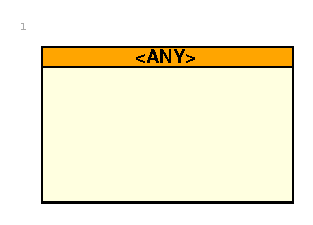
\includegraphics[width=2.50in]{Rule_1_LHS.eps}} &  $\rightarrow$&  \Ovalbox{ 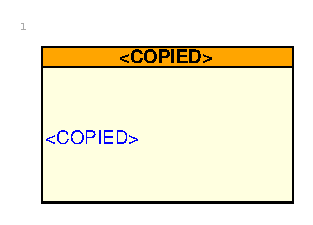
\includegraphics[width=2.50in]{Rule_1_RHS.eps}} \\
\end{tabular}}
\vspace{8pt}
\subsubsection*{Precondition: }
\begin{small}\begin{verbatim}
entity = self.getMatched(graphID, self.LHS.nodeWithLabel(1))
return entity.visited == 0
\end{verbatim}\end{small}

\hrule \vspace{6pt}
\subsubsection*{Post action: }
\begin{small}\begin{verbatim}
entity = self.getMatched(graphID, self.LHS.nodeWithLabel(1))
entity.visited = 1
posx, posy = 10+125*(self.graphRewritingSystem.NButtons%3), 10+70*(self.graphRewritingSystem.NButtons/3)
self.graphRewritingSystem.NButtons = self.graphRewritingSystem.NButtons + 1
ename = entity.name.toString()
file = self.graphRewritingSystem.file
file.write("   self.globalPrecondition(rootNode)\n\n")
file.write("   self.obj"+ename+"=ButtonConfig(self)\n")
file.write("   self.obj"+ename+".Contents.Text.setValue('New "+ename+"')\n")
file.write("   self.obj"+ename+".Contents.Image.setValue('')\n")
file.write("   self.obj"+ename+".Contents.lastSelected= 'Text'\n")
file.write("   self.obj"+ename+".Drawing_Mode.setValue(1)\n")
file.write("   self.obj"+ename+".Action.setValue(('ActionButton1', (['Python', 'OCL'], 1), ")
file.write("(['PREcondition', 'POSTcondition'], 1),")
file.write("(['EDIT', 'SAVE', 'CREATE', 'CONNECT', 'DELETE', 'DISCONNECT', 'TRANSFORM', 'SELECT', 'DRAG', 'DROP', 'MOVE OBJECT'], ")
file.write("[0, 0, 0, 0, 0, 0, 0, 0, 0, 0, 0]), ")
file.write("'# This method has as parameters:\\n")
file.write("#   - wherex : X Position in window coordinates where the user clicked.\\n")
file.write("#   - wherey : Y Position in window coordinates where the user clicked.\\n")
file.write("newPlace = self.createNew"+ename+" (self, wherex, wherey)\\n'))\n")
file.write("   self.obj"+ename+".graphClass_= graph_ButtonConfig\n")
file.write("   if self.genGraphics:\n")
file.write("      from graph_ButtonConfig import *\n")
file.write("      new_obj = graph_ButtonConfig("+str(posx)+", "+str(posy)+",self.obj"+ename+")\n")
file.write("      new_obj.DrawObject(self.UMLmodel)\n")
file.write("      self.UMLmodel.addtag_withtag('ButtonConfig', new_obj.tag)\n")
file.write("   else: new_obj = None\n")
file.write("   self.obj"+ename+".graphObject_ = new_obj\n")
file.write("   rootNode.addNode(self.obj"+ename+")\n")
file.write("   self.globalAndLocalPostcondition(self.obj"+ename+", rootNode)\n")
\end{verbatim}\end{small}

\hrule \vspace{6pt}

\hrule \vspace{6pt}
\section*{  Rule 2 (Order 2): buttonFromRelationship3}

\Ovalbox{
\begin{tabular}{ c c c  }
  LHS &  $\rightarrow$& RHS \\
   \Ovalbox{ 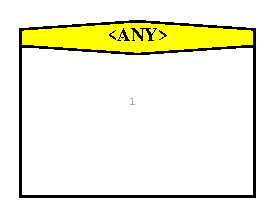
\includegraphics[width=2.50in]{Rule_2_LHS.eps}} &  $\rightarrow$&  \Ovalbox{ 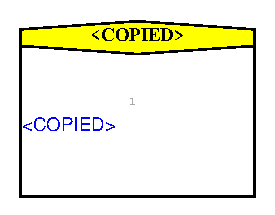
\includegraphics[width=2.50in]{Rule_2_RHS.eps}} \\
\end{tabular}}
\vspace{8pt}
\subsubsection*{Precondition: }
\begin{small}\begin{verbatim}
entity = self.getMatched(graphID, self.LHS.nodeWithLabel(1))
return entity.visited == 0
\end{verbatim}\end{small}

\hrule \vspace{6pt}
\subsubsection*{Post action: }
\begin{small}\begin{verbatim}
entity = self.getMatched(graphID, self.LHS.nodeWithLabel(1))
entity.visited = 1
ename = entity.name.toString()
posx, posy = 10+125*(self.graphRewritingSystem.NButtons%3), 10+70*(self.graphRewritingSystem.NButtons/3)
self.graphRewritingSystem.NButtons = self.graphRewritingSystem.NButtons + 1
file = self.graphRewritingSystem.file
file.write("   self.globalPrecondition(rootNode)\n\n")
file.write("   self.obj"+ename+"=ButtonConfig(self)\n")
file.write("   self.obj"+ename+".Contents.Text.setValue('New "+ename+"')\n")
file.write("   self.obj"+ename+".Contents.Image.setValue('')\n")
file.write("   self.obj"+ename+".Contents.lastSelected= 'Text'\n")
file.write("   self.obj"+ename+".Drawing_Mode.setValue(1)\n")
file.write("   self.obj"+ename+".Action.setValue(('ActionButton1', (['Python', 'OCL'], 1), ")
file.write("(['PREcondition', 'POSTcondition'], 1),")
file.write("(['EDIT', 'SAVE', 'CREATE', 'CONNECT', 'DELETE', 'DISCONNECT', 'TRANSFORM', 'SELECT', 'DRAG', 'DROP', 'MOVE OBJECT'], ")
file.write("[0, 0, 0, 0, 0, 0, 0, 0, 0, 0, 0]), ")
file.write("'# This method has as parameters:\\n")
file.write("#   - wherex : X Position in window coordinates where the user clicked.\\n")
file.write("#   - wherey : Y Position in window coordinates where the user clicked.\\n")
file.write("newPlace = self.createNew"+ename+" (self, wherex, wherey)\\n'))\n")
file.write("   self.obj"+ename+".graphClass_= graph_ButtonConfig\n")
file.write("   if self.genGraphics:\n")
file.write("      from graph_ButtonConfig import *\n")
file.write("      new_obj = graph_ButtonConfig("+str(posx)+", "+str(posy)+",self.obj"+ename+")\n")
file.write("      new_obj.DrawObject(self.UMLmodel)\n")
file.write("      self.UMLmodel.addtag_withtag('ButtonConfig', new_obj.tag)\n")
file.write("   else: new_obj = None\n")
file.write("   self.obj"+ename+".graphObject_ = new_obj\n")
file.write("   rootNode.addNode(self.obj"+ename+")\n")
file.write("   self.globalAndLocalPostcondition(self.obj"+ename+", rootNode)\n")
\end{verbatim}\end{small}

\hrule \vspace{6pt}

\hrule \vspace{6pt}
\hrule \vspace{6pt}
\subsubsection*{Global final action: }
\begin{small}\begin{verbatim}
file = self.rewritingSystem.file

file.write("newfunction = "+self.rewritingSystem.name+"\n")
file.write("loadedMMName = 'Buttons'\n")

for nt in graph.listNodes.keys():
 for node in graph.listNodes[nt]:
    del node.visited     

del self.rewritingSystem.file
del self.rewritingSystem.NButtons
\end{verbatim}\end{small}

\hrule \vspace{6pt}
\hrule \vspace{6pt}

\end{document}
